\documentclass[tikz,border=6mm]{standalone}
\usepackage{amsmath,amssymb}
\usetikzlibrary{arrows.meta,positioning,calc,fit,backgrounds}
% Minimal shared style library (vendored). Spacing: xs 4mm, sm 8mm, md 12mm, lg 20mm, xl 32mm.
% Line weights (ISO 128 series): light 0.7pt tertiary/dotted, regular 1.0pt borders + data/dashed,
% strong 1.4pt primary flow, emphasis 2.0pt one callout max. Weight = importance, spacing = grouping,
% dash = category. Every box pins BOTH minimum width and text width.
\def\wLight{0.7pt}\def\wRegular{1.0pt}\def\wStrong{1.4pt}\def\wEmph{2.0pt}
\definecolor{cTwin}{HTML}{2F855A}\definecolor{cLearn}{HTML}{2B6CB0}\definecolor{cBiz}{HTML}{B7791F}
\definecolor{cExec}{HTML}{805AD5}\definecolor{cNv}{HTML}{76B900}\definecolor{cInk}{HTML}{222222}
\tikzset{
  arch/.style={font=\sffamily, every node/.style={align=center}},
  box/.style={draw=cInk, line width=\wRegular, rounded corners=3pt, minimum height=1.05cm,
    minimum width=3.1cm, text width=2.7cm, font=\sffamily\small, fill=white},
  note/.style={font=\sffamily\scriptsize, text=black!60},
  twin/.style={box, fill=cTwin!10, draw=cTwin!80!black},
  learn/.style={box, fill=cLearn!10, draw=cLearn!80!black},
  biz/.style={box, fill=cBiz!14, draw=cBiz!80!black},
  exec/.style={box, fill=cExec!10, draw=cExec!80!black},
  base/.style={box, fill=black!6, draw=black!55},
  nv/.style={draw=cNv!80!black, line width=\wRegular, dotted, rounded corners=3pt, fill=cNv!8,
    minimum height=0.7cm, minimum width=7.4cm, text width=7.0cm, font=\sffamily\scriptsize},
  lane/.style={font=\sffamily\bfseries\scriptsize, text=black!55, anchor=east, text width=2.6cm, align=right},
  flow-a/.style={draw=cInk, line width=\wStrong, -{Stealth[length=2.6mm]}},
  flow-b/.style={draw=cLearn!70!black, line width=\wRegular, dashed, -{Stealth[length=2.6mm]}},
  flow-c/.style={draw=black!60, line width=\wLight, dotted, -{Stealth[length=2.2mm]}},
  flow-d/.style={draw=cExec!80!black, line width=\wRegular, dash dot, -{Stealth[length=2.4mm]}},
  eq/.style={font=\sffamily\scriptsize, text=black!55, fill=white, inner sep=1.5pt},
}
% math macros shared with the monograph
\providecommand{\V}{\mathcal{V}}\providecommand{\E}{\mathcal{E}}\providecommand{\Rel}{\mathcal{R}}
\providecommand{\N}{\mathcal{N}}\providecommand{\R}{\mathbb{R}}
\newcommand{\sub}[1]{{\sffamily\scriptsize\color{black!60}#1}}

\begin{document}
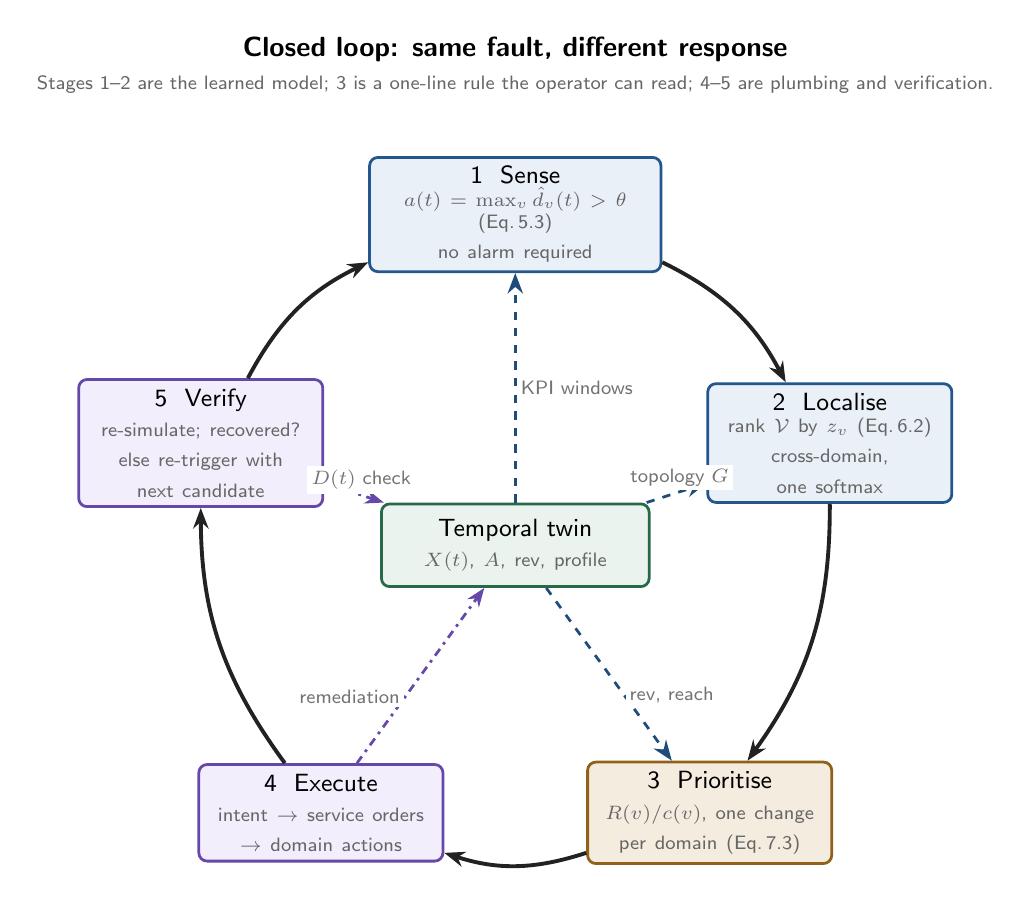
\begin{tikzpicture}[arch, x=1cm, y=1cm]
% Five stages on a ring (radius 4.2), one twin in the middle. Primary flow clockwise.
\def\Rr{4.2}
\node[box, fill=cTwin!10, draw=cTwin!80!black, minimum width=3.4cm, text width=3.0cm] (twin) at (0,0)
  {Temporal twin\\ \sub{$X(t)$, $A$, rev, profile}};
\node[learn, minimum width=3.7cm, text width=3.3cm] (sense) at (90:\Rr)  {1\ \ Sense\\ \sub{$a(t)=\max_v\hat d_v(t)>\theta$ (Eq.\,5.3)\\ no alarm required}};
\node[learn] (loc)   at (18:\Rr)  {2\ \ Localise\\ \sub{rank $\V$ by $z_v$ (Eq.\,6.2)\\ cross-domain, one softmax}};
\node[biz]   (prio)  at (-54:\Rr) {3\ \ Prioritise\\ \sub{$R(v)/c(v)$, one change per domain (Eq.\,7.3)}};
\node[exec]  (exe)   at (-126:\Rr){4\ \ Execute\\ \sub{intent $\to$ service orders $\to$ domain actions}};
\node[exec]  (ver)   at (162:\Rr) {5\ \ Verify\\ \sub{re-simulate; recovered? else re-trigger with next candidate}};
\draw[flow-a] (sense) to[bend left=18] (loc);
\draw[flow-a] (loc)   to[bend left=18] (prio);
\draw[flow-a] (prio)  to[bend left=18] (exe);
\draw[flow-a] (exe)   to[bend left=18] (ver);
\draw[flow-a] (ver)   to[bend left=18] (sense);
\draw[flow-b] (twin) -- (sense) node[eq, midway, right] {KPI windows};
\draw[flow-b] (twin) -- (loc)   node[eq, pos=0.55, above] {topology $G$};
\draw[flow-b] (twin) -- (prio)  node[eq, pos=0.62, right] {rev, reach};
\draw[flow-d] (exe)  -- (twin)  node[eq, pos=0.38, left] {remediation};
\draw[flow-d] (ver)  -- (twin)  node[eq, pos=0.62, above] {$D(t)$ check};
\node[font=\sffamily\bfseries] at (0, 6.3) {Closed loop: same fault, different response};
\node[note] at (0, 5.85) {Stages 1--2 are the learned model; 3 is a one-line rule the operator can read; 4--5 are plumbing and verification.};
\end{tikzpicture}
\end{document}
